\newpage
\section{Analisi di capacità} \label{ref:capacita}
Come è stato detto l'istituto ospedaliero Gaetano Pini oltre ad essere un istituto specializzato nella cura e nella riabilitazione di malattie ortopediche è anche un eccellenza nella ricerca universitaria. \\
Gli SLA definiti con l'azienda sono molto stringenti. In particolare è bene tenere presente che tutte le stime e le analisi si baseranno su bisogni del campo operativo dell'azienda, quello medico, che è molto delicato. In particolare si terranno presenti:
\begin{itemize}
	\item i requisiti delle norme UNI EN ISO 9001:2000;
	\item gli standards Joint Commission International;
	\item gli obiettivi e alle indicazioni fornite dalla programmazione nazionale, regionale e locale;
	\item per i servizi più critici il servizio dovrà essere disponibile 24/24.
\end{itemize}

\subsection{Modeling}
	Raccogliere informazioni sull'utilizzo e le performance dei vari servizi e tecnologie utilizzate dall'azienda è indispensabile per  ottenere una corretta pianificazione delle capacità. \\
	Questa attività è utilizzata a beneficio di molte attività, in particolare anche all'Availability Management. Per questo le descrizioni sottostanti sono riprese dal documento "Availability Plan" consegnato in allegato a questo documento.
	\subsubsection{Monitoring}
Utilizzando il monitoring ci assicuriamo che i servizi IT siano disponibili, eseguano in conformità con gli SLA e quindi mantengano il livello di servizio concordato. Nella sua forma base, un processo di monitoring invia un segnale ad un asset IT quale server, router, etc.. e si aspetta un segnale di ritorno per capire se la risorsa IT stia funzionando o meno.
Ad un livello superiore è invece utile avere informazioni più dettagliate sull'esecuzione di una componente IT, per esempio il livello di occupazione di CPU di un dato server.\\
Viene qui utilizzato un tool di Real Time Monitoring che permette di monitorare lo stato attivo e presente dell'ambiente IT attraverso una continua e costante collezione di dati e accessi. \\
Per il monitoring abbiamo utilizzato AppOptics che ci permette di monitorare attivamente sia l'infrastruttura che le applicazioni IT.
\subsubsection{Trend Analysis}
Monitorare per un lungo periodo di tempo i livelli di availability dell'infrastruttura IT attraverso un tool di monitoring e salvare quei dati su di grafici, ci consente di avere delle buone stime della disponibilità dei vari servizi IT ed inoltre di identificare in un maniera proattiva dei potenziali problemi prima che essi si verifichino. Purtroppo affinchè questa tecnica sia efficace è necessario aspettare un lungo periodo di tempo per raccogliere varie informazioni e far si che le previsioni siano il più attendibili possibile.\\
Ciò è stato realizzato attraverso il tool di monitoring AppOptics ed al suo modulo di reportage e grafici mensili.
\subsection{Previsione dell'utilizzo e delle prestazioni del servizio}
	Per una dettagliata analisi delle risorse IT necessarie è bene che i servizi IT che vengono utilizzati dall'istituto (che sono stati descritti nella sezione \ref{ref:scenario.applicativi}, precisamente nella tabella \ref{tab:applicativi}) siano identificati attraverso il loro utilizzo da parte degli utenti e le loro performace. \\

	\subsubsection{Presupposti}
	Le performace analizzate in questa sezione riguardano l'utilizzo medio dei servizi da parte degli utenti, senza considerare quindi picchi improvvisi e sovraccarichi, incidenti o malfunzionamenti hardware o software. \\
	\subsubsection{Previsioni}
	L'analisi dei servizi tutt'ora proposti insieme alle previsioni di crescita del volume di business ha portato alla definizione di un piano di crescita per i servizi IT.\\
	In dettaglio:
	\begin{itemize}
		\item l'aumento del numero di utenti prevista è dettato da un incremento del personale;
		\item l'aumento degli utenti attivi è dettato da un aumento dei pazienti;
		\item l'aumento delle performance è dovuto al miglioramento dell'infrastruttura tecnologica che ha portato ad un'ottimizzazione, ad un calo degli incidenti e delle interruzioni di servizio.
	\end{itemize}

Inoltre si vuole precisare che le performance per ogni servizio sono calcolate in base a valori dati da:
\begin{itemize}
	\item efficienza del servizio,
	\item efficacia del servizio,
	\item il raggiungimento degli SLA specifici del servizio
\end{itemize}
La soglia minima di performance raggiunta si attesta all’85\%, al di sopra di quanto concordato negli SLA. 

\newpage
	
	Nella tabella \ref{tab:analisiServizi} vengono identificati i servizi IT, il loro utilizzo da
parte degli utenti attuale e quello previsto per il prossimo anno, il numero di utenti e le loro performance attuali e previste.
	\begin{table}[h!]
	\begin{tabular}{|c|C{3cm}|| C{1.5cm} |C{1.5cm} ||C{1.5cm} | C{1.5cm} || C{1.5cm}| C{1.5cm}|}
		\hline
		\rowcolor[HTML]{EFEFEF} 
		\textbf{N} & \textbf{Sistema applicativo}  & \textbf{N. utenti} & \textbf{N. utenti previsti} & \textbf{N. utenti attivi}  & \textbf{N. utenti attivi previsti} & \textbf{Performance di servizio} & \textbf{Performance di servizio previste} \\ \hline
		1  & Archivio Clinico		& 15	& 20	& 10	& 13  & 80\%	& 90\%	\\ \hline
		2  & Argos			        	&5	& 8	& 2	& 4 & 70\%	& 85\%	\\ \hline
		3  & Armonia					&6	& 8	& 3	& 4 & 90\%	& 95\%	\\ \hline
		4  & Emonet						& 10	& 15	&2	& 3 &	85\%	& 90\%	\\ \hline
		5  & Aurora Web				& 650	& 800	&100	& 150 &	 85\% &	90\%	\\ \hline
		6  & Gst\_est					& 650	& 800	& 20 & 35 &	80\%& 	85\%	\\ \hline
		7  & Gst\_fat					& 6	&	8 &4	& 6 & 70\%	& 80\%	\\ \hline
		8  & Pacs						& 49	& 55	& 20	& 30	& 90\%	& 95\%	\\ \hline
		9  & Elefante					& 49	& 60	& 20	& 35 &	85 & 	95\%	\\ \hline
		10  & Ormawin2000		& 6	& 8	& 3	& 4 & 75\%	& 	85\%	\\ \hline
		11  & PowerLab				& 10	& 15	& 5	& 7 & 90\%	& 	95\%	\\ \hline
		12  & Rap						& 6	& 7	&	4& 5 &80\%	& 90\%		\\ \hline
		13  & Ican						& 350	& 450	&100	& 150 &	80\%& 	90\%	\\ \hline
		14  & Aliseo					& 20	& 35	&5	& 12 & 90\%	& 	95\%	\\ \hline
		15  & Enco					& 43	& 50	&20	& 25 & 75\%	& 	85\%	\\ \hline
		16  & Teseo						& 10	& 15	&2	& 5 & 70\%	& 	\%85	\\ \hline
		17  & Protocollo			& 15	& 20	& 5	& 10 & 85\%	& 	90\%	\\ \hline
	\end{tabular}
\caption{Analisi servizi IT}\label{tab:analisiServizi}
\end{table}
	
\newpage
\subsection{Previsione dell'utilizzo e delle prestazioni delle risorse} \label{ref:previsione.risorse}
In questa sezione vengono analizate le infrastrutture tecnologiche esistenti e le loro performance che sono stati descritti nella sezione \ref{ref:scenario.tecnologie}, basandoci sulle previsioni fatte. \\
	\subsubsection{Presupposti}
	Le performace analizzate in questa sezione riguardano l'utilizzo medio dei servizi da parte degli utenti (e quindi delle varie tecnologie), senza considerare quindi picchi improvvisi e sovraccarichi, incidenti o malfunzionamenti hardware o software.
	
\subsubsection{Calcolo delle stime}
Per calcolare le performance delle tecnologie IT sono stati considerati vari parametri di seguito definiti:
\paragraph{CPU}
Il calcolo del numero di unità di CPU necessarie è stato fatto in base al numero di utenti medio giornaliero:\\
\begin{figure}[h!]
	\centering
	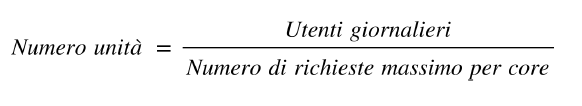
\includegraphics[width=0.5\linewidth]{./img/cpu}
\end{figure}

\paragraph{RAM}
La quantità di RAM da allocare ed è stata
decisa in base alla complessità del servizio nel quale viene utilizzata.

\paragraph{Storage}
La quantità di spazio di archiviazione invece è stata calcolato stimando la dimensione media dei file e il numero di utenti che utilizzano quel determinato servizio. \\
\begin{figure}[h!]
	\centering
	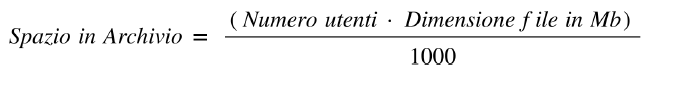
\includegraphics[width=0.5\linewidth]{./img/archivio}
\end{figure}

\subsubsection{Previsioni}
	Le stime di incremento della capacità necessarie a garantire quanto concordato nei SLA sono state fatte rispetto all’incremento delle utenze per l'aumento dei dipendenti e dei pazienti previsto nel prossimo anno.
In particolare è stato rilevato un aumento del:
\begin{itemize}
	\item 5\% di capacità computazionale (RAM) media;
	\item 10\% di memoria per unità computazionale;
	\item 10\% di archiviazione per i servizi.
\end{itemize}
È quindi necessario incrementare conseguentemente la capacità dell’infrastruttura
concordemente alle percentuali di incremento calcolate.


	\paragraph{Server}
	La prima considerazione da effettuare riguarda il rinnovamento dell'hardware: è preferibile procedere con la sostituzione dei sistemi più critici invece che con il miglioramento di essi tramite integrazioni. Questo perchè in caso di malfunzionamenti e/o guasti la riparazione potrebbe essere difficile, i pezzi da sostituire potrebbero non essere ancora in commercio o comunque di difficile reperibilità rischiando così di allungare i tempi e i costi. \\
	Nella tabella sottostante ritroviamo il numero e la tipologia di server da acquistare per sostituire gli hardware più critici:
	\begin{table}[h]
		\centering
		\begin{tabular}{|C{2cm} | C{10cm} |} 
			\hline
			\rowcolor[HTML]{EFEFEF} 
			\textbf{Quantità}  & \textbf{Server} \\ \hline
			3 & Rack server one socket   \\ \hline
			2 & Server di livello industriale   \\ \hline
		\end{tabular}
		\caption{Analisi nuovi server}\label{tab:analisiServer}
	\end{table}
	
	Per i server più recenti, invece, è bene procedere con un miglioramento delle prestazioni in modo da assicurare i livelli concordati dallo SLA. Di seguito troviamo una tabella che riassume le attività di incremento delle quantità e delle performance dei server che si occupano di mantenere i servizi attivi.\\
		Gli incrementi hardware previsti serviranno ad un miglioramento dei servizi sul lato prestazionale. \\
	In particolare per ogni tipologia di server abbiamo:
	\begin{itemize}
		\item Quantità di server presenti e tutt'ora e quantità prevista per ottenere le performace di servizio per gli applicativi analizzati nella tabella \ref{tab:analisiServizi};
		\item numero di CPU attuali e previste nel piano;
		\item RAM attuale e prevista;
		\item storage attuale e previsto.
	\end{itemize}
	\begin{table}[h]
		\centering
		\begin{tabular}{|C{2cm} || C{1.5cm} | C{1.5cm}|| C{1.5cm} |C{1.5cm} || C{1.5cm} |C{1.5cm}|| C{1.5cm} |C{1.5cm}|} 
			\hline
			\rowcolor[HTML]{EFEFEF} 
			\textbf{Server}  &\textbf{Quantità attuale} &\textbf{Quantità prevista} & \textbf{CPU attuale} & \textbf{CPU prevista} & \textbf{RAM attuale} & \textbf{RAM prevista} & \textbf{Storage attuale} & \textbf{Storage previsto} \\ \hline
			Applicazione RAP & 2 & 3 & 2& 2& 32GB & 32GB & 512GB& 1TB \\ \hline
			Disaster Recovery & 1 & 1 & 2 & 2& 16GB& 16GB &2TB&4TB\\ \hline
			Test & 1 & 1& 2 &  2& 16GB& 32GB& 512GB&512GB\\ \hline
		\end{tabular}
	\end{table}

	\begin{table}[h]
	\centering
	\begin{tabular}{|C{2cm} || C{1.5cm} | C{1.5cm}|| C{1.5cm} |C{1.5cm} || C{1.5cm} |C{1.5cm}|| C{1.5cm} |C{1.5cm}|} 
		\hline
		\rowcolor[HTML]{EFEFEF} 
		\textbf{Server}  &\textbf{Quantità attuale} &\textbf{Quantità prevista} & \textbf{CPU attuale} & \textbf{CPU prevista} & \textbf{RAM attuale} & \textbf{RAM prevista} & \textbf{Storage attuale} & \textbf{Storage previsto} \\ \hline
		DataBase & 2 & 3 & 2 & 4 & 16 GB & 16GB & 2TB& 3TB\\ \hline
		Application Server & 2 & 3 & 2 & 4 & 16GB&32GB & 244GB& 1TB\\ \hline
		Porta Applicativa SISS & 2 & 3 & 2 & 2& 16GB & 16GB & 1TB& 2TB \\ \hline
	\end{tabular}
	\caption{Analisi server attuali}\label{tab:analisiServer}
\end{table}

\paragraph{Backup}
Per quanto riguarda il raggiungimento dello SLA per la disponibilità del servizio 24 ore su 24 è stato stimato che i server disponibili al momento non sono sufficienti per assicurare ciò. \\
Oltre al numero di server aggiuntivi affiancati a quelli tutt'ora presenti già esaminati nel precedente paragrafo si è preso in esame la virtualizzazione di un sistema del backup, anche per non tenere sistemi di backup e di produzione nello stesso rank. \\
In dettaglio è bene procedere con l'acquisto di:
\begin{itemize}
	\item n. 4 nodi computazionali 
	\item licenza VMware
\end{itemize}